\documentclass{article}
\usepackage[margin=1in]{geometry}
\usepackage{tikz}
\usetikzlibrary{shapes.geometric, arrows, positioning}
%For tikz node diagram setup
\pagenumbering{gobble}

\definecolor{mgreen}{HTML}{689562}
\definecolor{mpurp}{HTML}{85678f}
\definecolor{mblue}{HTML}{3C406C}
\definecolor{mgray}{HTML}{6F6F6F}
\tikzset{trapezium stretches=true}
\tikzstyle{source} = [rectangle, rounded corners, minimum width= 2cm, minimum height = 1cm, text = white, text centered, fill = mgray]
\tikzstyle{input} = [trapezium, trapezium left angle=50, trapezium right angle = 130, minimum width = 1.5cm, minimum height=1cm, text centered, text=white, fill=mgreen]
\tikzstyle{routing} = [diamond, minimum width=2cm, minimum height=1cm, aspect = 2, text width = 2cm, text centered, text=white,fill = mblue]
\tikzstyle{processor} = [rectangle, minimum width = 2cm, minimum height = 1cm, text width = 3cm, text = white, fill = mpurp]
\tikzstyle{cable} = [thick, ->, >=latex]
\tikzstyle{usb} = [thick, <->, >=latex]


\begin{document}
\centering
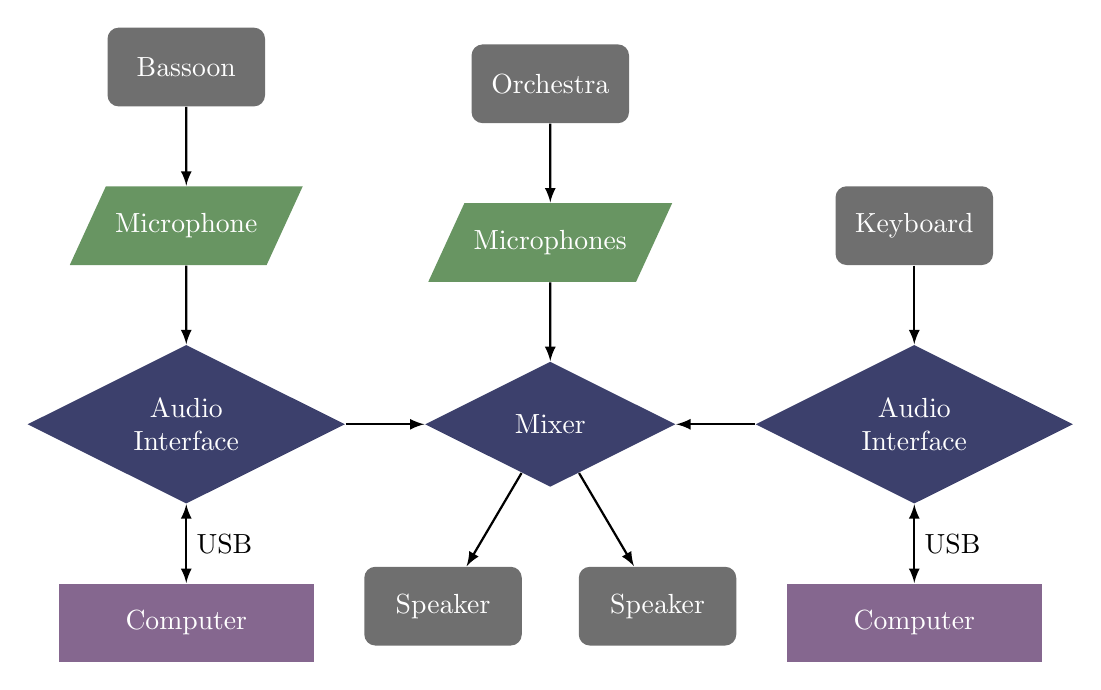
\begin{tikzpicture}[align=center, node distance = 1cm]
\node (mix) [routing] {Mixer};
\node (int1) [routing, left = of mix] {Audio Interface};
\node (int2) [routing, right = of mix] {Audio Interface};
\node (comp1) [processor, below = of int1] {Computer};
\node (comp2) [processor, below = of int2] {Computer};
\node (speaker1) [source, below = of mix, xshift = -9ex] {Speaker};
\node (speaker2) [source, below = of mix, xshift = 9ex] {Speaker};
\node (mic1) [input, above= of int1] {Microphone};
\node (mic2) [input, above= of mix] {Microphones};
\node (orch) [source, above= of mic2] {Orchestra};
\node (bsn) [source, above= of mic1] {Bassoon};
\node (keys) [source, above = of int2] {Keyboard};
\draw [cable] (bsn) -- (mic1);
\draw [cable] (mic1) -- (int1);
\draw [cable] (orch) -- (mic2);
\draw [cable] (mic2) -- (mix);
\draw [cable] (keys) -- (int2);
\draw [usb] (int1) -- node[anchor=west] {USB}(comp1);
\draw [usb] (int2) -- node[anchor=west] {USB}(comp2);
\draw [cable] (int1) -- (mix);
\draw [cable] (int2) -- (mix);
\draw [cable] (mix) -- (speaker1);
\draw [cable] (mix) -- (speaker2);
\end{tikzpicture}


\end{document}
